\documentclass{standalone}
\usepackage{tikz}
\usepackage{color}
\usetikzlibrary{positioning, shapes, arrows.meta, calc}
\definecolor{myblue}{RGB}{63, 99,136}
\definecolor{myred}{RGB}{168, 50, 50}

\begin{document}
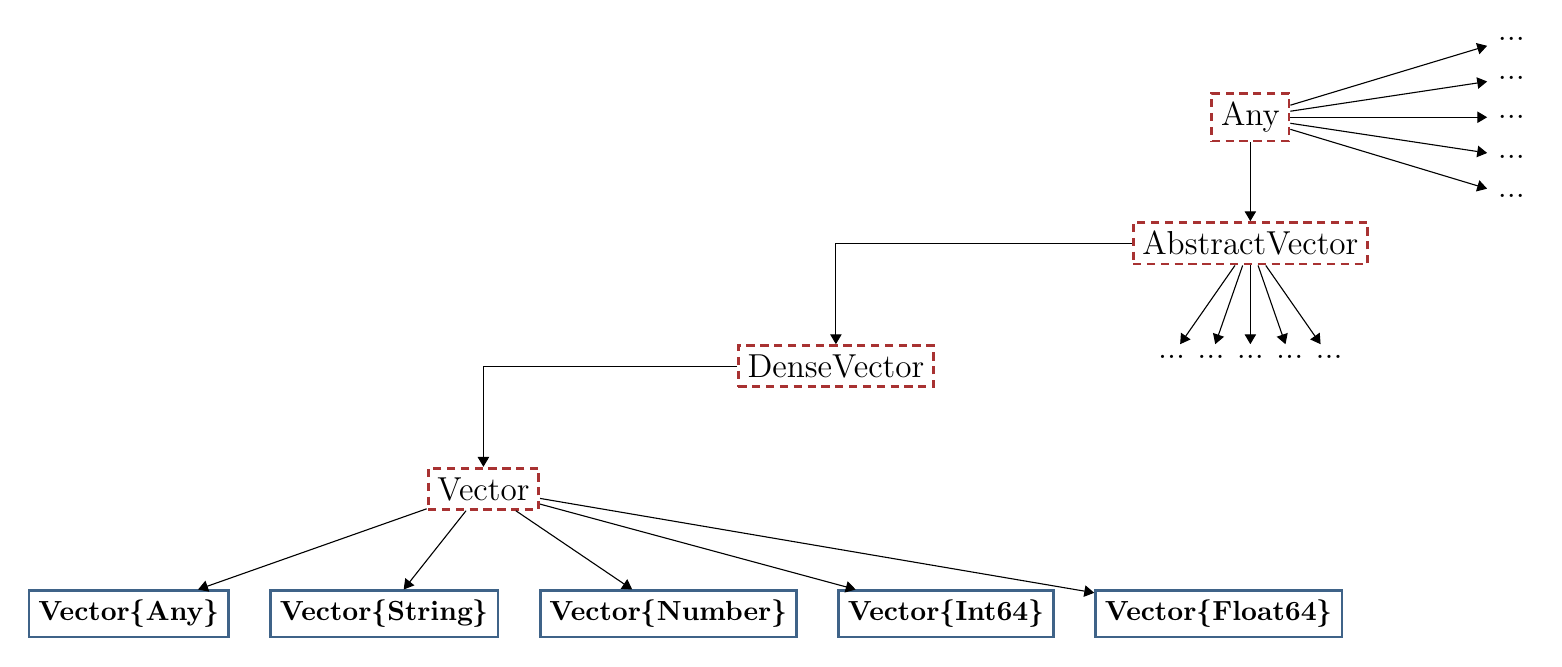
\begin{tikzpicture}[
   every node/.style       = {font=\large},
    node distance            = 1cm and 2.5cm,
         concreteNode/.style = {rectangle, align=center, draw= myblue, line width=1, font=\bfseries},
         abstractNode/.style = {rectangle, draw=myred, align=center, line width=1, densely dashed},
         otherNode/.style = {rectangle, align=center, line width=1, densely dashed},
         myarrow/.style      = {-Triangle}
]



\node[abstractNode] (any) {Any};
\node[otherNode, right=of any, yshift=0cm, xshift=-0.0cm] (others) {...};
\node[otherNode, right=of any, yshift=0.5cm, xshift=-0.0cm] (otherss) {...};
\node[otherNode, right=of any, yshift=1.0cm, xshift=-0.0cm] (othersss) {...};
\node[otherNode, right=of any, yshift=-0.5cm, xshift=-0.0cm] (otherssss) {...};
\node[otherNode, right=of any, yshift=-1.0cm, xshift=-0.0cm] (othersssss) {...};
\draw[myarrow] (any)  -- (others);
\draw[myarrow] (any)  -- (otherss);
\draw[myarrow] (any)  -- (othersss);
\draw[myarrow] (any)  -- (otherssss);
\draw[myarrow] (any)  -- (othersssss);

    \node[abstractNode, below=of any, yshift=0cm, xshift=-0.0cm] (abstract) {AbstractVector};
    \node[abstractNode, below left=of abstract, yshift=0cm, xshift=-0.0cm] (dense) {DenseVector};
    \node[abstractNode, below left=of dense, yshift=-0cm, xshift=-0cm] (vector) {Vector};

    \draw[myarrow] (any)  -- (abstract);
    \draw[myarrow] (abstract)  -| (dense);
    \draw[myarrow] (dense) -| (vector);

        

        

    
    \node[concreteNode, below left=of vector, xshift=0cm] (int128) {Vector\{Any\}};
     \node[concreteNode, right=of int128, xshift=-2cm] (int64) {Vector\{String\}};
    \node[concreteNode, right=of int64,xshift=-2cm] (int32) {Vector\{Number\}};
    \node[concreteNode, right=of int32,xshift=-2cm] (int16) {Vector\{Int64\}};
    \node[concreteNode, right=of int16,xshift=-2cm] (int8) {Vector\{Float64\}};
    

    
    \draw[myarrow] (vector) -- (int128);
    \draw[myarrow] (vector) -- (int64);
    \draw[myarrow] (vector) --(int32);
    \draw[myarrow] (vector) -- (int16);
    \draw[myarrow] (vector) -- (int8);
    


\node[otherNode, below=of abstract, yshift=0cm, xshift=-0.0cm]   (cothers) {...};
\node[otherNode, below=of abstract, yshift=0.0cm, xshift=0.5cm] (cotherss) {...};
\node[otherNode, below=of abstract, yshift=0.0cm, xshift=1.0cm] (cothersss) {...};
\node[otherNode, below=of abstract, yshift=-0.0cm, xshift=-0.5cm] (cotherssss) {...};
\node[otherNode, below=of abstract, yshift=-0.0cm, xshift=-1.0cm] (cothersssss) {...};
\draw[myarrow] (abstract)  -- (cothers);
\draw[myarrow] (abstract)  -- (cotherss);
\draw[myarrow] (abstract)  -- (cothersss);
\draw[myarrow] (abstract)  -- (cotherssss);
\draw[myarrow] (abstract)  -- (cothersssss);
    
\end{tikzpicture}
\end{document}
